\documentclass{article}
\usepackage{graphicx}
\usepackage[utf8]{inputenc}
\usepackage{amsmath, amssymb, latexsym}

\usepackage{pgfplots}
\usepackage{algorithm}
\usepackage[noend]{algpseudocode}
\usepackage{tikz}
\usepackage{nicefrac}
\pgfplotsset{every axis legend/.append style={
at={(0,0)},
anchor=north east}}
\usetikzlibrary{shapes,positioning,intersections,quotes}
\usetikzlibrary{arrows.meta,
                bending,
                intersections,
                quotes,
                shapes.geometric}
                
\definecolor{darkgreen}{rgb}{0.0, 0.6, 0.0}
\definecolor{darkred}{rgb}{0.7, 0.0, 0.0}
\makeatletter
\makeatother
\begin{document}


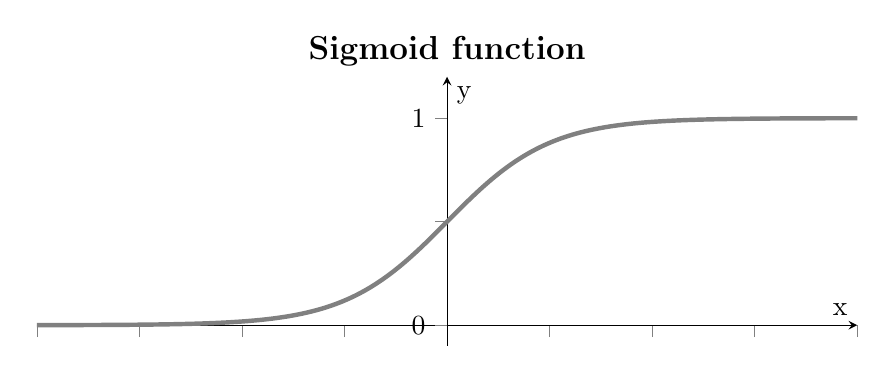
\begin{tikzpicture}
  \begin{axis}[
      axis x line=middle,
      axis y line=middle,
      width=12cm, height=5cm,     % size of the image
      grid = none,
      grid style={dashed, gray!0},
      %xmode=log,log basis x=10,
      %ymode=log,log basis y=10,
      xmin= -8,     % start the diagram at this x-coordinate
      xmax= 8,    % end   the diagram at this x-coordinate
      ymin=-0.1,     % start the diagram at this y-coordinate
      ymax= 1.2,   % end   the diagram at this y-coordinate
      %/pgfplots/xtick={0,1,...,60}, % make steps of length 5
      %extra x ticks={23},
      extra y ticks={0, 1},
      axis background/.style={fill=white},
      ylabel=y,
      xlabel=x,
      xticklabels={,,},
      yticklabels={,,},
      tick align=outside,
      tension=0.08]
    % plot the stirling-formulae
    \addplot[domain=-8:8, gray, ultra thick,samples=500] {1/(1+exp(-x)};

  \end{axis}
  \node[above,font=\large\bfseries] at (current bounding box.north) {Sigmoid function
  };
\end{tikzpicture}


\end{document}